%        File: arfc-beamer.tex
%     Created: Sun May 5 10:00 PM 2013 C
%


%\documentclass[11pt,handout]{beamer}
\documentclass[9pt]{beamer}
\usetheme[white]{Illinois}
%\title[short title]{long title}
\title[Cyclus, an agent-based fuel cycle simulator]{Cyclus, an agent-based fuel cycle simulator}
%\subtitle[short subtitle]{long subtitle}
\subtitle[Brief Overview]{Brief Overview}
%\author[short name]{long name}
\author[Jin Whan Bae, Kathryn Huff]{Jin Whan Bae, Kathryn Huff}
%\date[short date]{long date}
\date[05.21.2018]{May 21, 2018}
%\institution[short name]{long name}
\institute[UIUC]{University of Illinois at Urbana-Champaign}

%%%% Acronym support

\usepackage[acronym,toc]{glossaries}
\newacronym{NNL}{NNL}{National Nuclear Laboratory}
\newacronym{MA}{MA}{minor actinide}
\newacronym{DU}{DU}{depleted uranium}
\newacronym{LWR}{LWR}{Light Water Reactor}
\newacronym{MOX}{MOX}{Mixed Oxide Fuel}
\newacronym{SFR}{SFR}{Sodium-cooled Fast Reactor}
\newacronym{FLM}{FLM}{Fuel Loading Model}
\newacronym{EFMC}{EFMC}{Effective fissile mass coefficient}
\newacronym{ORNL}{ORNL}{Oak Ridge National Laboratory}
\newacronym{PWR}{PWR}{Pressurized Water Reactor}
\newacronym{FIT}{FIT}{Functionality Isolation Test}

\makeglossaries

%\usepackage{bbding}
\usepackage{amsfonts}
\usepackage{lipsum}
\usepackage{adjustbox}
\usepackage{fancyvrb}
\usepackage{amsmath}
\usepackage{xspace}
\usepackage{graphicx}
\usepackage{subfigure}
\usepackage{listings}
\usepackage{booktabs} % nice rules for tables
\usepackage{microtype} % if using PDF
\usepackage{bigints}
\DeclareMathOperator{\erf}{erf}
%I need some complimentary error funcitons... 
\DeclareMathOperator{\erfc}{erfc}
%page numbers
\setbeamertemplate{footline}[page number]
\setbeamertemplate{caption}[numbered]
%Those icons in the references are terrible looking
\setbeamertemplate{bibliography item}[text]


%try to get rid of header on title page\dots
\makeatletter
    \newenvironment{withoutheadline}{
        \setbeamertemplate{headline}[default]
        \def\beamer@entrycode{\vspace*{-\headheight}}
    }{}
\makeatother



\newcommand\blfootnote[1]{%
  \begingroup
  \renewcommand\thefootnote{}\footnote{#1}%
  \addtocounter{footnote}{-1}%
  \endgroup
}

\usepackage{booktabs} % nice rules (thick lines) for tables
\usepackage{microtype} % improves typography for PDF
\usepackage{xspace}
\usepackage{tabularx}
\usepackage[affil-it]{authblk}
\usepackage{tikz}

\usepackage{tikz}
\usetikzlibrary{positioning, arrows, decorations, shapes}

\usetikzlibrary{shapes.geometric,arrows}
\tikzstyle{process} = [rectangle, rounded corners, minimum width=3cm, minimum height=1cm,text centered, draw=black, fill=blue!30]
\tikzstyle{object} = [ellipse, rounded corners, minimum width=3cm, minimum height=1cm,text centered, draw=black, fill=green!30]
\tikzstyle{arrow} = [thick,->,>=stealth]

\usepackage{cleveref}
\usepackage{datatool}
\newcolumntype{b}{X}
\newcolumntype{s}{>{\hsize=.5\hsize}X}
\newcolumntype{m}{>{\hsize=.75\hsize}X}

\newcommand{\Cyclus}{\textsc{Cyclus}\xspace}%
\graphicspath{ {images/} }
\usetikzlibrary{positioning, arrows, decorations, shapes }

\begin{document}
%%%%%%%%%%%%%%%%%%%%%%%%%%%%%%%%%%%%%%%%%%%%%%%%%%%%%%%%%%%%%
%% From uw-beamer Here's a handy bit of code to place at 
%% the beginning of your presentation (after \begin{document}):
\newcommand*{\alphabet}{ABCDEFGHIJKLMNOPQRSTUVWXYZabcdefghijklmnopqrstuvwxyz}
\newlength{\highlightheight}
\newlength{\highlightdepth}
\newlength{\highlightmargin}
\setlength{\highlightmargin}{2pt}
\settoheight{\highlightheight}{\alphabet}
\settodepth{\highlightdepth}{\alphabet}
\addtolength{\highlightheight}{\highlightmargin}
\addtolength{\highlightdepth}{\highlightmargin}
\addtolength{\highlightheight}{\highlightdepth}
\newcommand*{\Highlight}{\rlap{\textcolor{HighlightBackground}{\rule[-\highlightdepth]{\linewidth}{\highlightheight}}}}
%%%%%%%%%%%%%%%%%%%%%%%%%%%%%%%%%%%%%%%%%%%%%%%%%%%%%%%%%%%%%
%%--------------------------------%%
\begin{withoutheadline}
\frame{
  \titlepage
}
\end{withoutheadline}

%%--------------------------------%%

\section{Before We Start}
\begin{frame}
	\frametitle{Agent-based Framework}
	\begin{itemize}
		\item Cyclus is agent-based, which means it's very modular
		\item User can develop / plug in facilities
			\begin{itemize}
				\item User can `design' their own fuel cycle
				\item Highly customizable
			\end{itemize}
	\end{itemize}
	\begin{figure}[htbp!]
        \begin{center}
                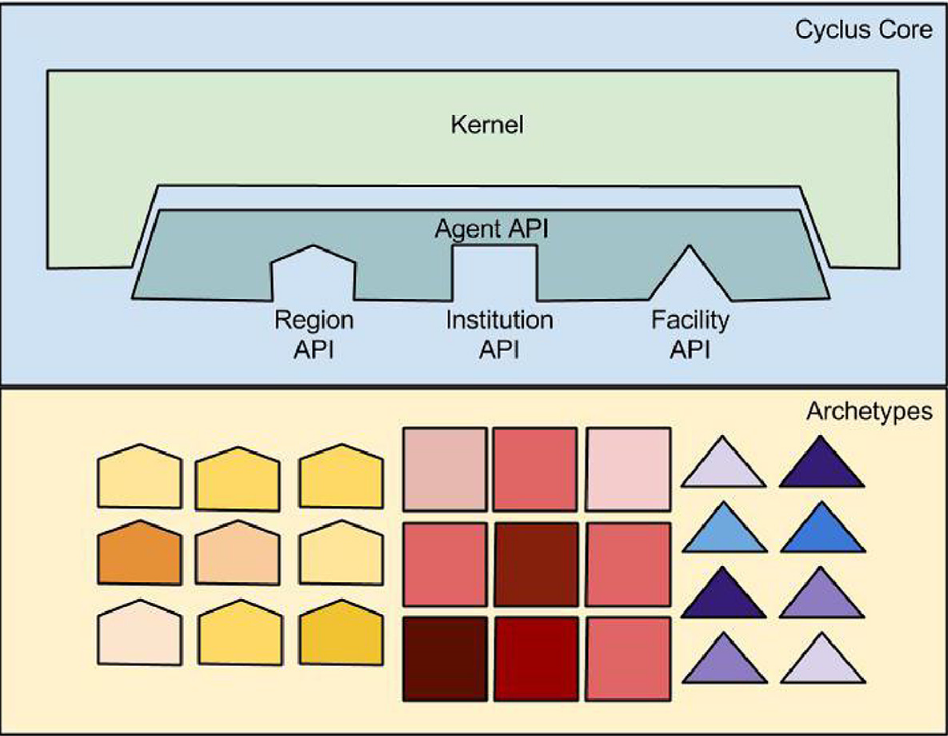
\includegraphics[width=.6\textwidth]{./images/cyclus_structure.png}
        \end{center}
        \caption{Modular Design of Cyclus}
        \label{fig:cyclus_struc}

	\end{figure}
\end{frame}

\begin{frame}
	\frametitle{Agent-based Framework}
	\begin{figure}[htbp!]
        \begin{center}
                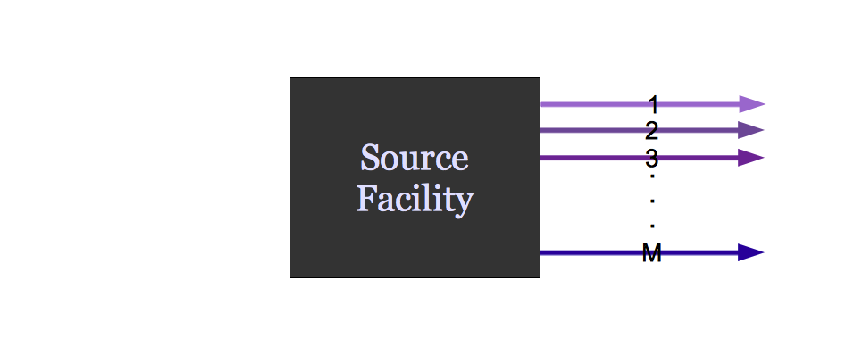
\includegraphics[width=\textwidth]{./images/source.png}
        \end{center}
	\end{figure}
\end{frame}

\begin{frame}
	\frametitle{Agent-based Framework}
	\begin{figure}[htbp!]
        \begin{center}
                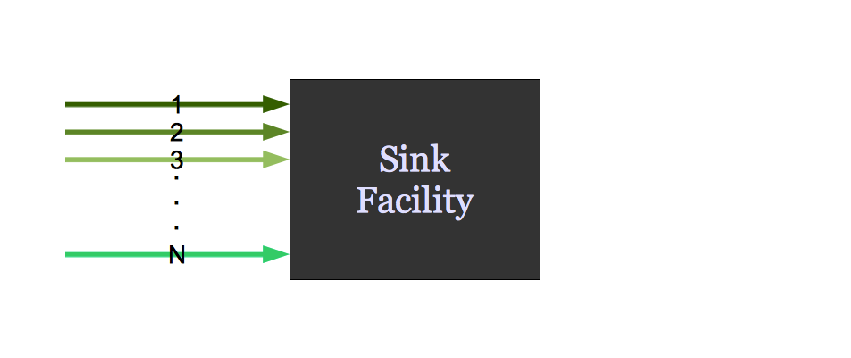
\includegraphics[width=\textwidth]{./images/sink.png}
        \end{center}
	\end{figure}
\end{frame}

\begin{frame}
	\frametitle{Agent-based Framework}
	\begin{figure}[htbp!]
        \begin{center}
                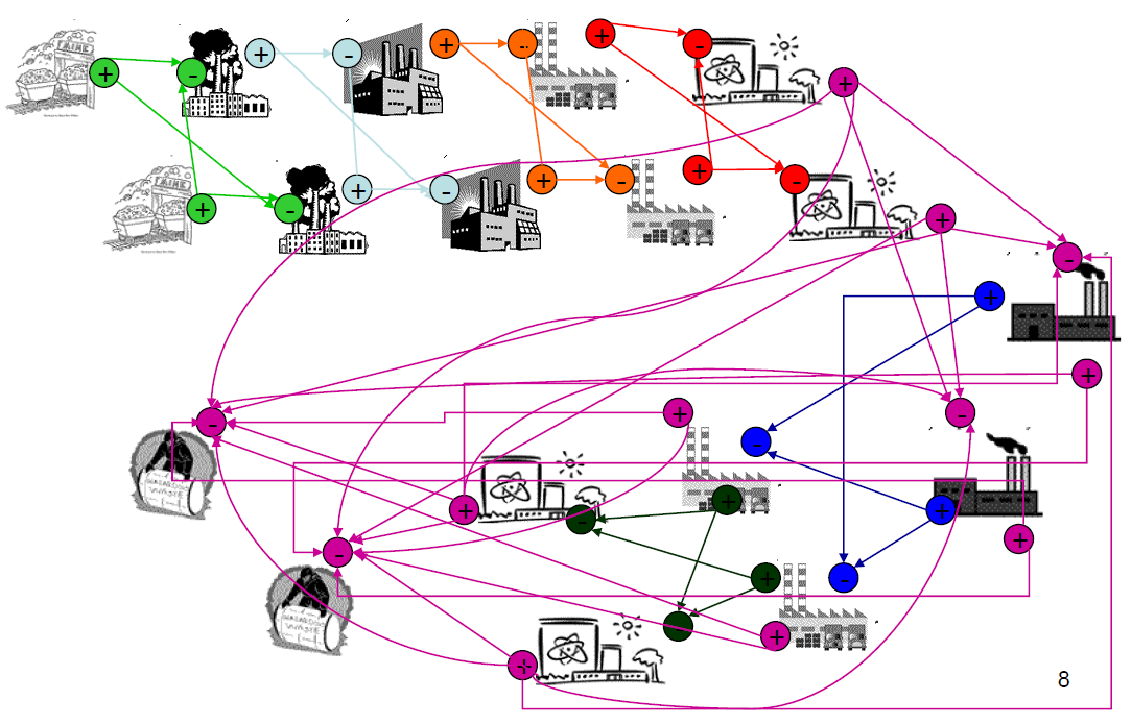
\includegraphics[width=\textwidth]{./images/flow.png}
        \end{center}
	\end{figure}
\end{frame}


\begin{frame}
    \frametitle{Timestep Execution}
    A simplified explanation: Each timestep:
    
\begin{figure}[H]
\centering
\scalebox{0.7}{
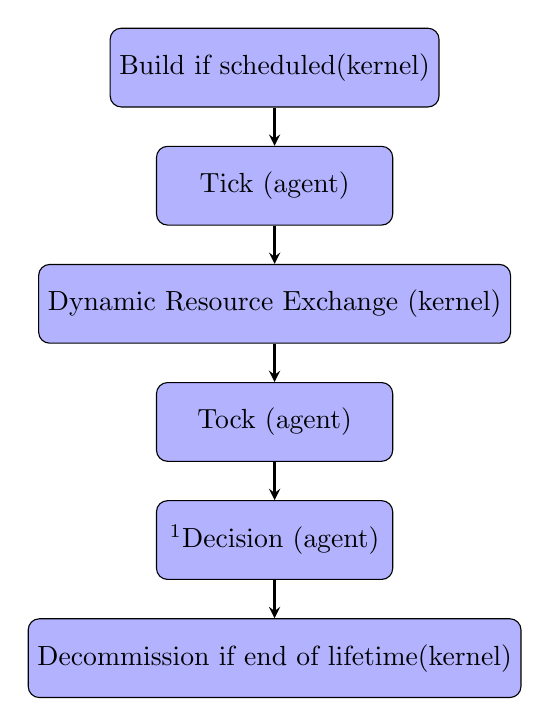
\begin{tikzpicture}[node distance=1.5cm]
\node (Build) [process] {Build if scheduled(kernel)};
\node (Tick) [process, below of=Build] {Tick (agent)};
\node (DRE) [process, below of=Tick]{Dynamic Resource Exchange (kernel) };
\node (Tock) [process, below of=DRE]{Tock (agent)};
\node (Decision) [process, below of=Tock] {\footnotemark Decision (agent)};
\node (Decom) [process, below of=Decision] {Decommission if end of lifetime(kernel)};

\draw [arrow] (Build) -- (Tick); 
\draw [arrow] (Tick) -- (DRE);
\draw [arrow] (DRE) -- (Tock);
\draw [arrow] (Tock) -- (Decision);
\draw [arrow] (Decision) -- (Decom);
\end{tikzpicture}
}
\end{figure}

\footnotetext{Decision phase is planned to be added in the next release.}
\end{frame}

\begin{frame}
	\frametitle{Terminology}
	\begin{itemize}
		\item \textbf{Archetypes}: A collection of logic and behavior which can be configured into a prototype which can then be instantiated in simulation as a agent. Archetypes are represented as C++ classes that inherit from the base cyclus::Agent class. (e.g. Reactor module, Sink module)
		\item \textbf{Prototypes}: Archetype + parameters (e.g. Reactor with input-defined  \texttt{name, cycle time, assembly size, core size etc})
		\item \textbf{Agents}: Every single `entity' in play during simulation (Region, Institution, Facility)
	\end{itemize}
\end{frame}

\begin{frame}
	\frametitle{Terminology}
	Agents can take the form of:
	\begin{itemize}
		\item \textbf{Region}: The largest agent that is a collection of institutions (Set trade /material constraints)
		\item \textbf{Institution}: Agent that manages facilities (Can deploy, decommission facilities)
		\item \textbf{Facility}: The agent that `trades' and does calculations (Trades material and transmutes, separates)
	\end{itemize}
\end{frame}

\begin{frame}
	\frametitle{Extensions - Archetypes}
	Since Cyclus is an extensible framework, anyone can develop a new archetype and plug-and-play. (\textcolor{blue}{Institution}, \textcolor{red}{region}, facility otherwise.)
	\begin{itemize}
		\item Cycamore: Sink, Storage, Recipe Reactor, Fuelfab, Enrichment, Source, \textcolor{blue}{DeployInst}, Mixer, Separations, \textcolor{red}{GrowthRegion} \cite{huff_fundamental_2016}
		\item \textcolor{blue}{$^*$D3ploy}: Demand-driven deployment Institution \cite{noauthor_d3ploy:_2018} 
		\item $^*$CYBORG: Reactor depletion analysis tool using ORIGEN \cite{skutnik_cyborg:_2016}
		\item $^*$CYDER: A CYclus Disposal Environment and Repository object \cite{huff_cyclus_2013}
		\item $^*$CORRM: Continuous On-line Reprocessing Reactor Module \cite{recycle_recycle:_2018}
		\item $^*$Pyre: Pyroprocessing module with non-proliferation metrics \cite{westphal_signatures_2018}
        \item $^*$Peddler: Simulate trucks and transport material between facilities \cite{noauthor_peddler:_2018}
		\item And more..
	\end{itemize}
    \blfootnote{$^*$ Third party module in active development.}
\end{frame}

\begin{frame}
	\frametitle{Extensions - Analysis / Drivers}
	There are other tools to help visualization / output data analysis of Cyclus.
	\begin{itemize}
		\item RICKSHAW: Automated stochastic driver for Cyclus
		\item Cymetric: Extracts important fuel cycle metrics
		\item Analysis: Collection of functions to extract metrics (e.g. natU usage, trade between two facilities, etc.) 
		\item Cycmap: GIS visualization tool for Cyclus
		\item Cyclist: GUI for Cyclus (depracated)
	\end{itemize}
\end{frame}


\begin{frame}
	\frametitle{Installation - Binary}
	Better, more thorough explanations are in \texttt{fuelcycle.org}
	\begin{itemize}
		\item Windows: Windows 10 support Experimental (Can use virtualbox) 
		\item MacOS: \texttt{conda install -c conda-forge cyclus cycamore}
		\item Linux: \texttt{conda install cyclus cycamore}
	\end{itemize}
\end{frame}


\begin{frame}
	\frametitle{Installation - Build from Source}
    All source files are open-source, and available on Github.

	\texttt{github.com/cyclus/cyclus} and \texttt{github.com/cycamore/cycamore} has the source files, and guides
	\begin{enumerate}
		\item Clone repository (\texttt{git clone [url]})
		\item Install dependency (see github guide README)
		\item \texttt{python install.py}
	\end{enumerate}

	\begin{figure}[htbp!]
        \begin{center}
                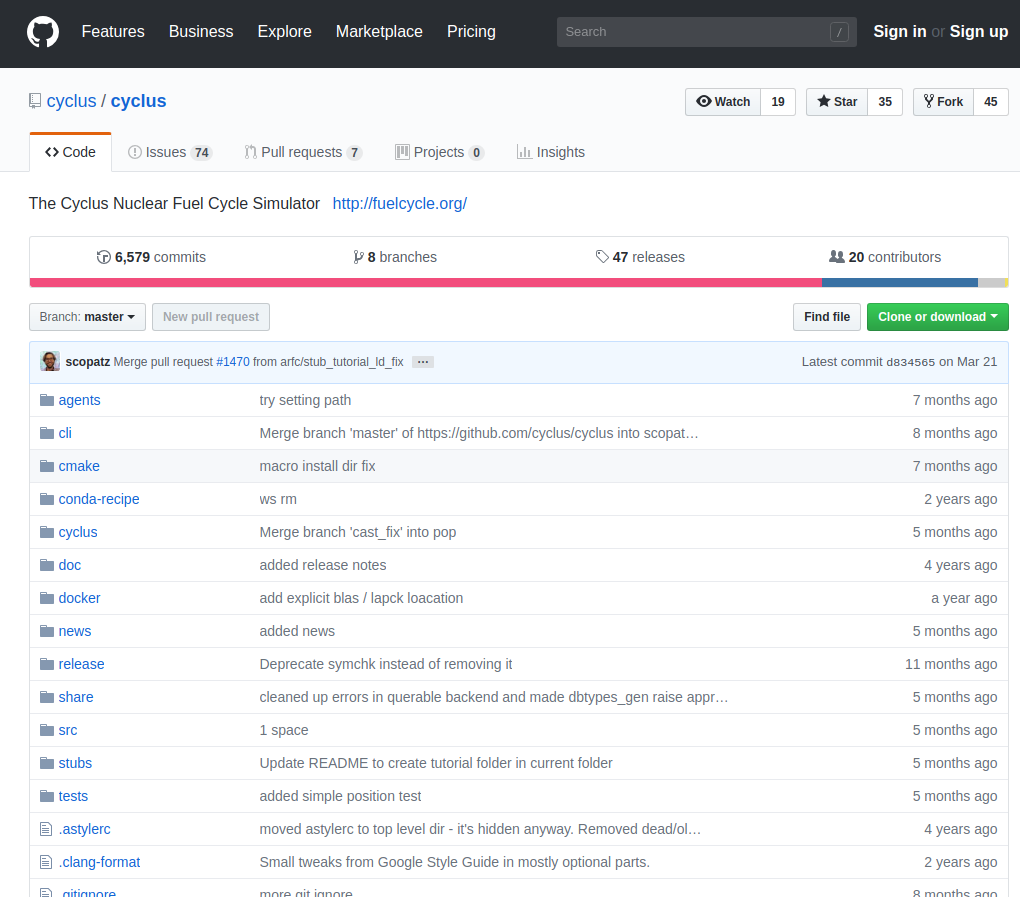
\includegraphics[width=.6\textwidth]{./images/github.png}
        \end{center}
        \caption{Github website for Cyclus}
	\end{figure}
\end{frame}


\begin{frame}
	\frametitle{Installation - TroubleShooting}
	Look for your error message or make a new post in the following Cyclus communities:
	\begin{enumerate}
		\item Github Issue in \texttt{github.com/cyclus/cyclus}
		\item Cyclus google user group
	\end{enumerate}
\end{frame}

\begin{frame}
	\frametitle{General Info}
	\begin{itemize}
		\item Written in: C++, Python
		\item Input file: Plaintext format (.xml, .json, .python)
		\item Output file: Database (.sqlite, .hdf5)
	\end{itemize}
\end{frame}




\section{Running Simulations}
\begin{frame}
    \frametitle{Structure}
    \begin{enumerate}
        \item \texttt{Control}: Simulation Definition
        \item \texttt{Archetypes}: List of available archetypes
        \item \texttt{Facility}: Facility prototypes - define parameters of archetypes
        \item \texttt{Region}: Region agents
        \item \texttt{Institution}: Institution agents (inside Region definition)
        \item \texttt{Recipe}: recipe definitions
    \end{enumerate}
\end{frame}

\begin{frame}
    \frametitle{Control}
\begin{figure}[htbp!]
        \begin{center}
                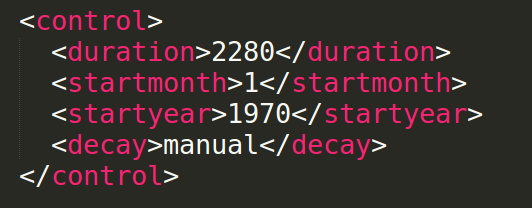
\includegraphics[width=.8\textwidth]{./images/control.png}
        \end{center}
    \end{figure}

\end{frame}

\begin{frame}
    \frametitle{Archetypes}
\begin{figure}[htbp!]
        \begin{center}
                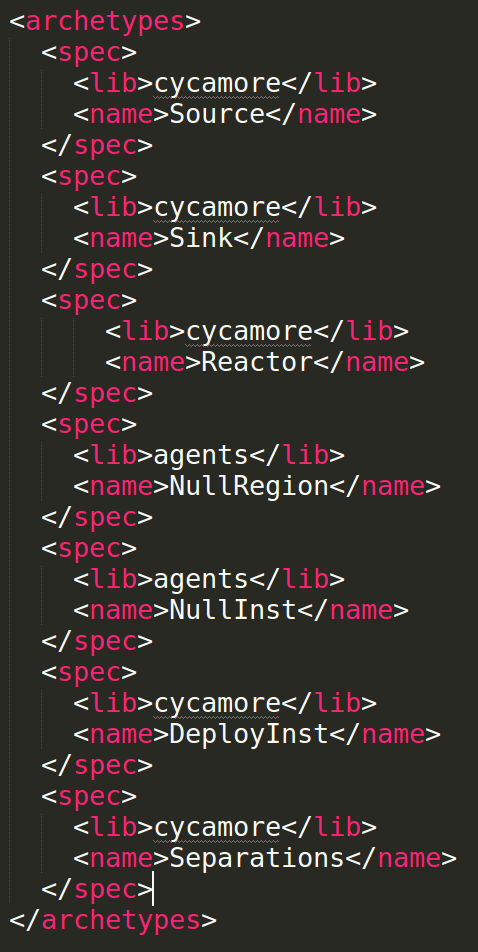
\includegraphics[height=.8\textheight]{./images/archetypes.png}
        \end{center}
    \end{figure}

\end{frame}

\begin{frame}
    \frametitle{Facility - Cycamore::Separations}
\begin{figure}[htbp!]
        \begin{center}
                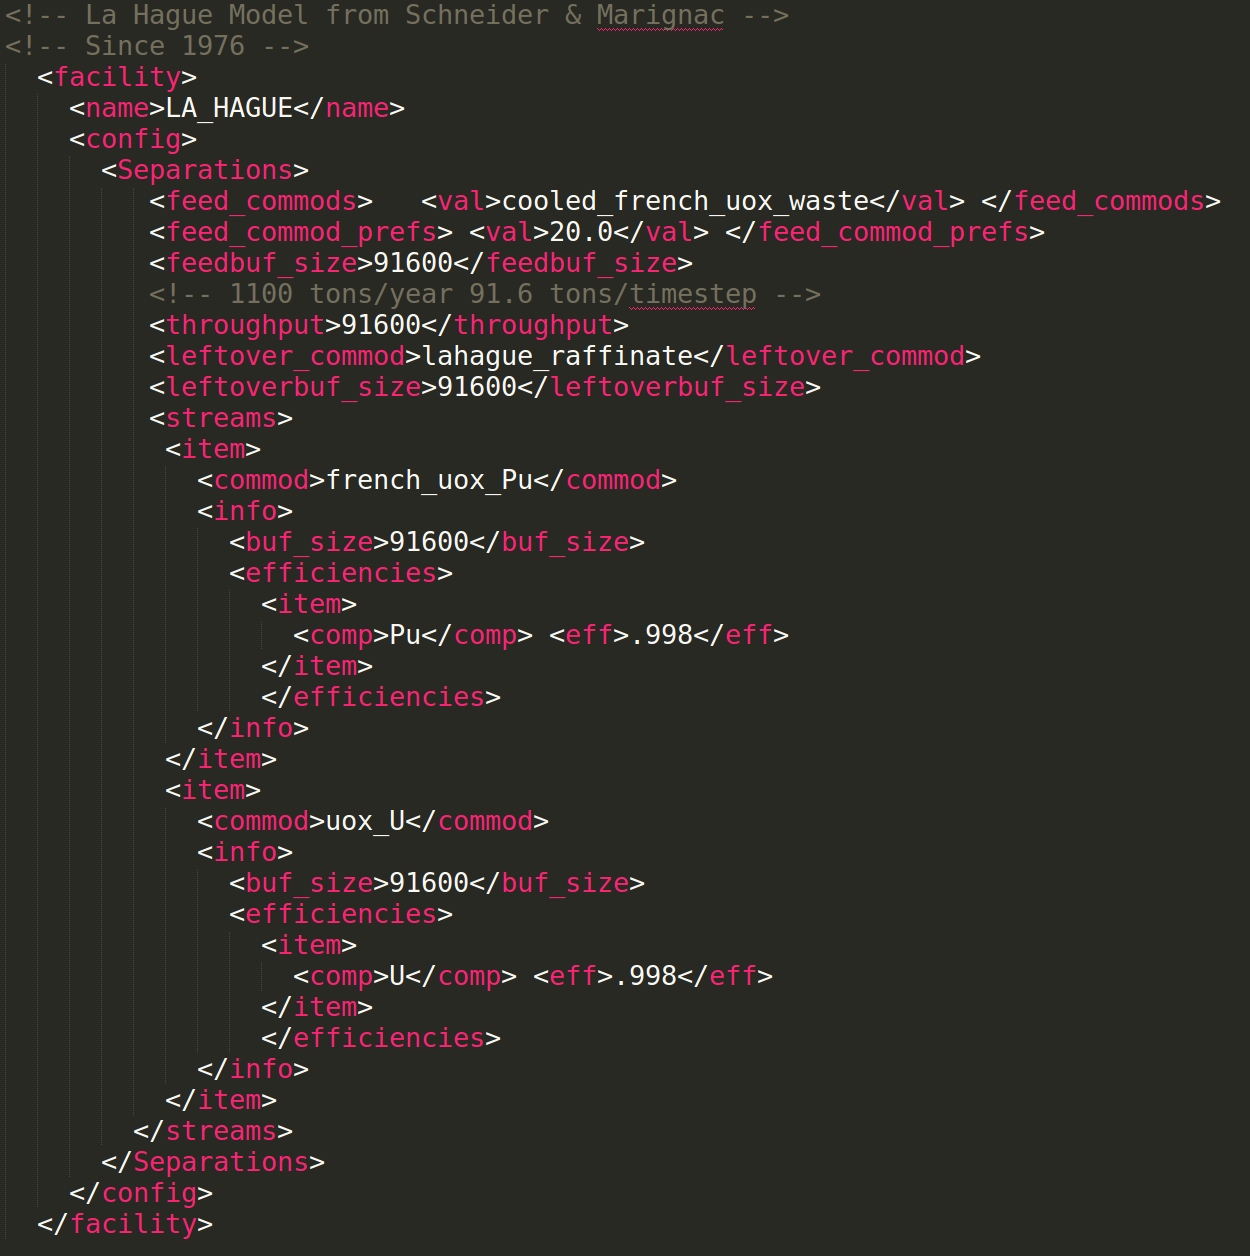
\includegraphics[width=.7\textwidth]{./images/lahague.png}
        \end{center}
    \end{figure}

\end{frame}

\begin{frame}
    \frametitle{Facility - Cycamore::Reactor}
\begin{figure}[htbp!]
        \begin{center}
                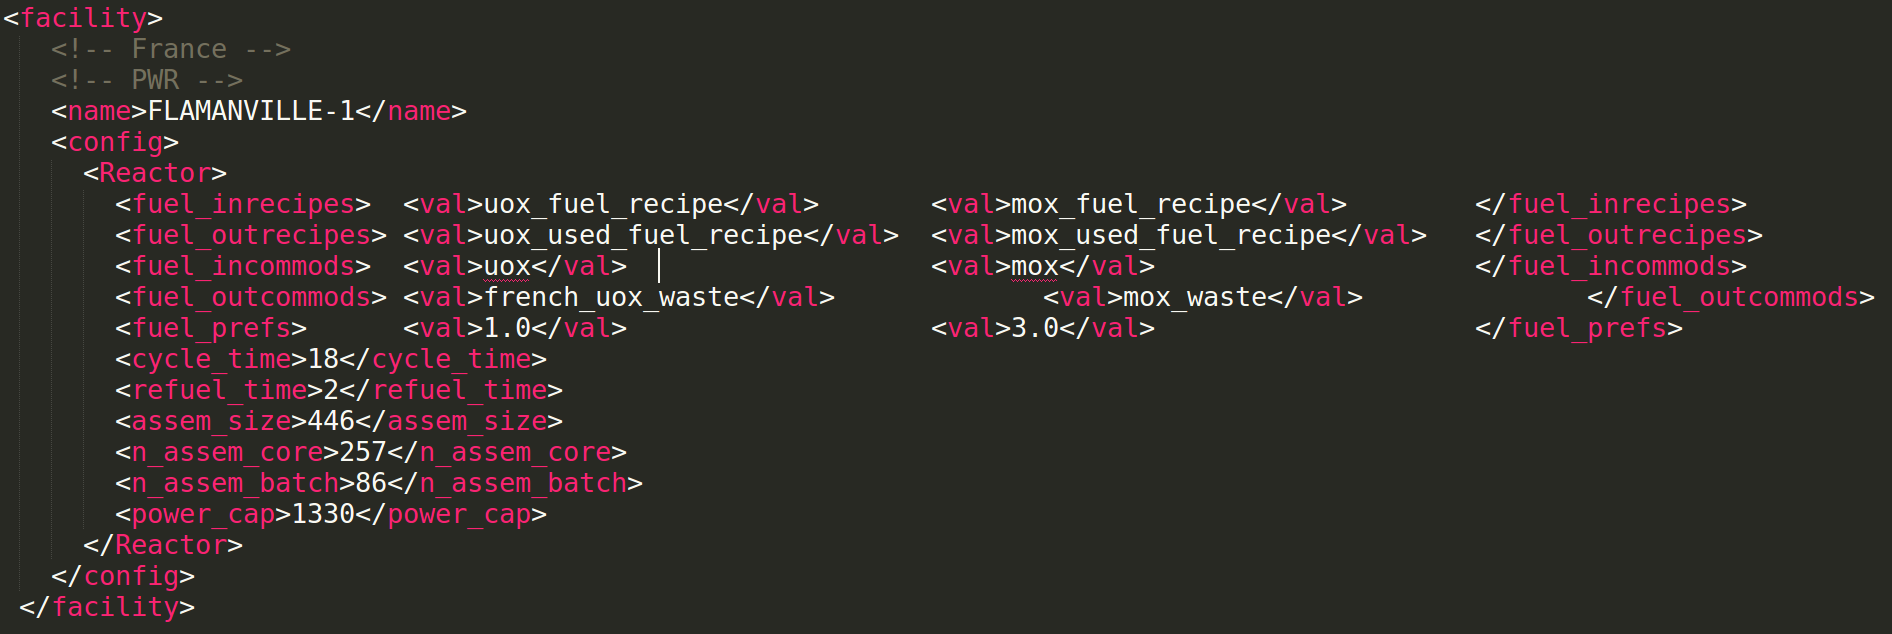
\includegraphics[width=1.1\textwidth]{./images/flamanville.png}
        \end{center}
    \end{figure}

\end{frame}

\begin{frame}
    \frametitle{Region}
\begin{figure}[htbp!]
        \begin{center}
                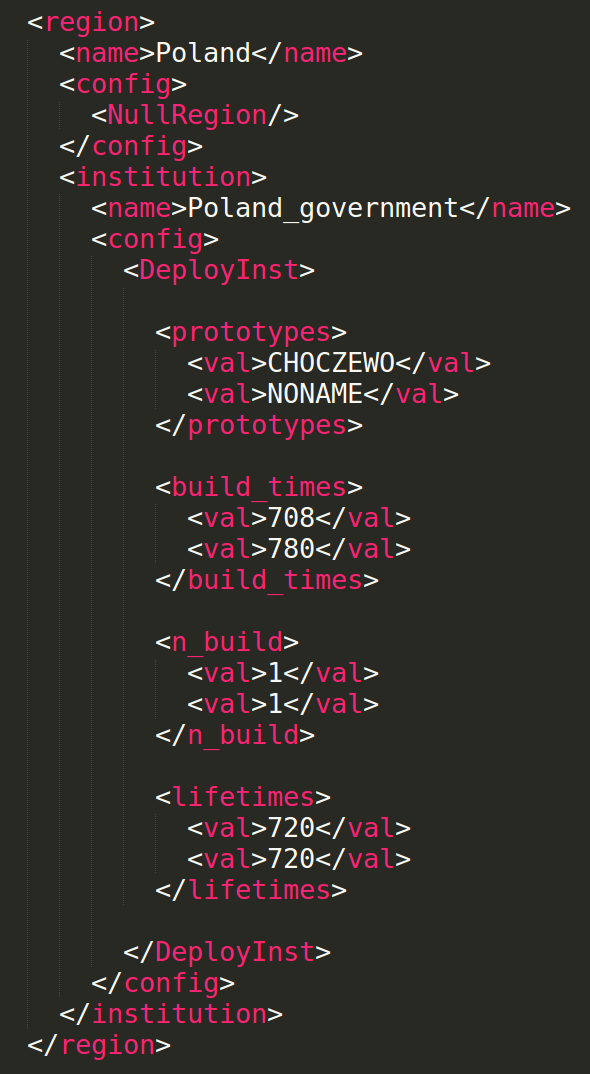
\includegraphics[height=.8\textheight]{./images/region.png}
        \end{center}
    \end{figure}

\end{frame}

\begin{frame}
    \frametitle{Recipe}
\begin{figure}[htbp!]
        \begin{center}
                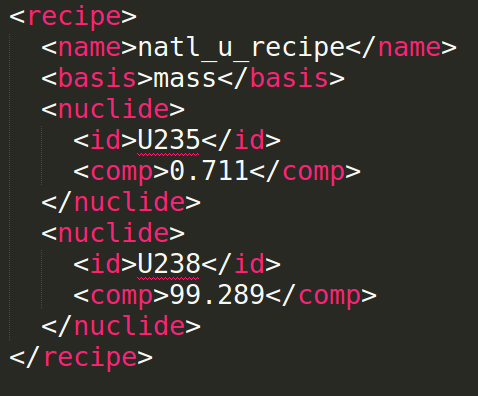
\includegraphics[width=.8\textwidth]{./images/recipe.png}
        \end{center}
    \end{figure}
\end{frame}


\begin{frame}
    \frametitle{Benefits}
    \begin{enumerate}
        \item Generate input file from database
        \begin{itemize}
            \item Reactor specifications from database
            \item Recipe from database
            \item Sensitivity study using external driver (e.g. RAVEN)
        \end{itemize}
        \item Simple automation / modification of input file
    \end{enumerate}
\end{frame}



\section{Output and Examples}
\begin{frame}
    \frametitle{Output}
    Developers can set what values to output for each archetype.
    Cyclus records all transactions between \texttt{Facilities}
    and other metrics unique to each archetype, such as:
    \begin{itemize}
        \item Cycamore::Reactor - Power generation per timestep
        \item Cycamore::Enrichment - SWU per timestep
    \end{itemize}
\end{frame}


\subsection{Example - French Transition}
\begin{frame}
    \frametitle{Example Workflow}
    This workflow was used in the paper \texttt{Synergistic Spent Nuclear Fuel Dynamics Within the European Union} (in ANS 2017 Winter meeting, journal publication submitted).

\begin{figure}
\scalebox{0.65}{
        \centering
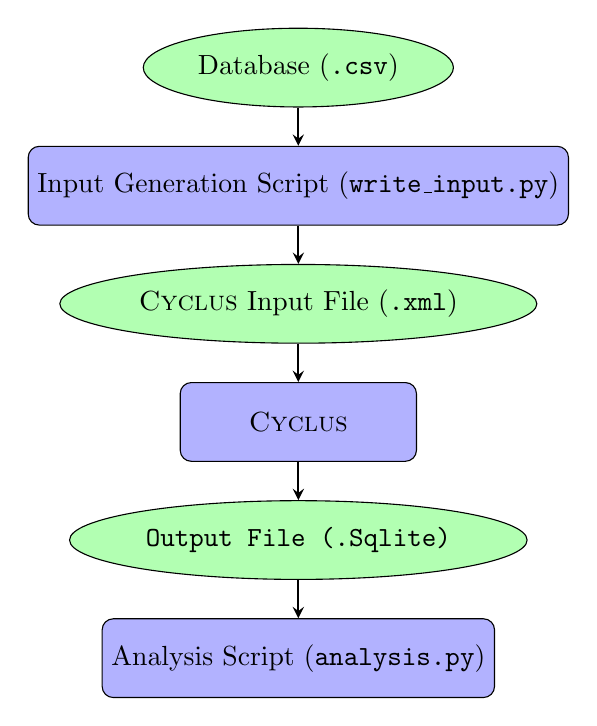
\begin{tikzpicture}[node distance=1.5cm]
\node (database) [object] {Database (\texttt{.csv})};
\node (script) [process, below of=database] {Input Generation Script (\texttt{write\_input.py})};
\node (input) [object, below of=script] {\Cyclus Input File (\texttt{.xml})};
\node (cyclus) [process, below of=input]{\Cyclus};
\node (output) [object, below of=cyclus]{\texttt{Output File (\texttt{.Sqlite})}};
\node (script2) [process, below of=output]{Analysis Script (\texttt{analysis.py})};

\draw [arrow] (database) -- (script); 
\draw [arrow] (script) -- (input); 
\draw [arrow] (input) -- (cyclus);
\draw [arrow] (cyclus) -- (output);
\draw [arrow] (output) -- (script2);
\end{tikzpicture}
}
\caption{Green circles and blue boxes represent files and software 
processes, respectively, in the computational workflow.}
\label{diag:comp}
\end{figure}

\end{frame}

\begin{frame}
    \frametitle{CSV to Cyclus input file}
    \begin{enumerate}
        \item Python script to parse through CSV file (reactor name, start / decom date, power output, etc)
        \item Use templates to construct input file (Python script fills curly brackets)
    \end{enumerate}
    \begin{figure}[htbp!]
        \begin{center}
                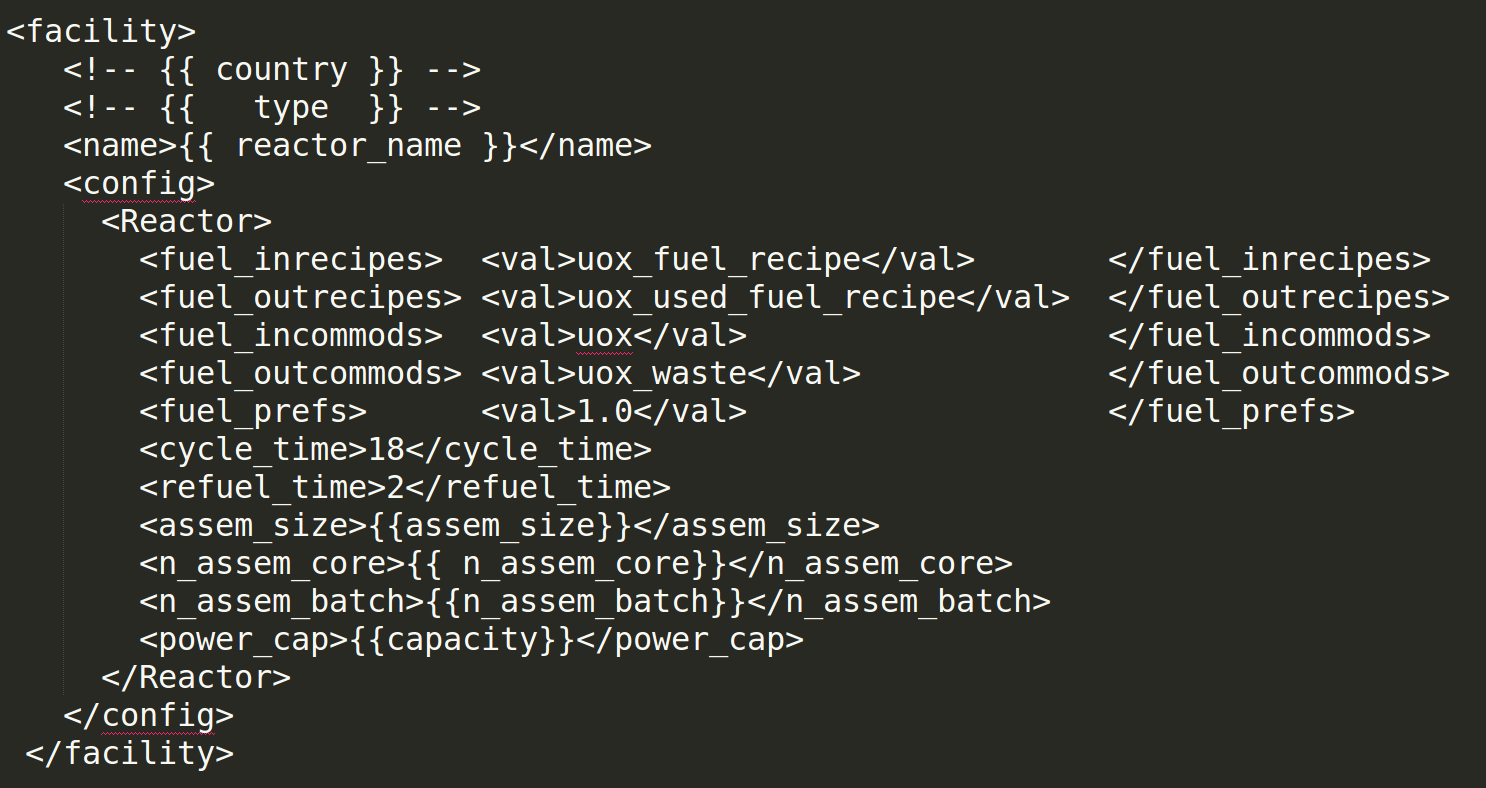
\includegraphics[width=.8\textwidth]{./images/reactor_template.png}
        \end{center}
    \end{figure}
\end{frame}

\begin{frame}
    \frametitle{Output analysis}
    \begin{itemize}
        \item Python script to query and process output data
        \item Use Jupyter notebook to organize / visualize output
    \end{itemize}
\end{frame}

\begin{frame}
    \frametitle{Scenario Description}
    \begin{itemize}
        \item France transitions from LWR fleet to SFR fleet
        \item France receives UNF from other EU nations for plutonium
    \end{itemize}
\end{frame}

\begin{frame}
    \frametitle{Output - regional analysis}
    \begin{itemize}
        \item The user can separate analysis by regions
        \item Concept of children-parent: each \texttt{facility} has a parent \texttt{Institution}, and each \texttt{Institution} has a parent \texttt{Region}.
    \end{itemize}
    \begin{figure}[htbp!]
        \begin{center}
                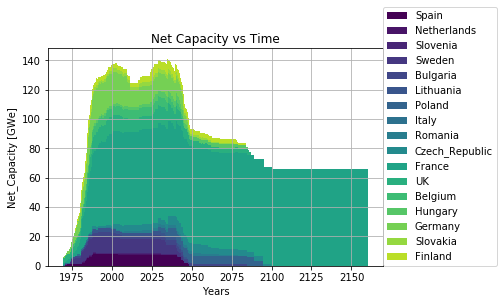
\includegraphics[width=.8\textwidth]{./images/sim_output/france/onesim.png}
        \end{center}
    \caption{Power generation is separated by region.}
    \end{figure}
\end{frame}

\begin{frame}
    \frametitle{Output - regional analysis}
    \begin{itemize}
        \item The user can separate analysis by regions
        \item Concept of children-parent: each \texttt{facility} has a parent \texttt{Institution}, and each \texttt{Institution} has a parent \texttt{Region}.
    \end{itemize}
    \begin{figure}[htbp!]
        \begin{center}
                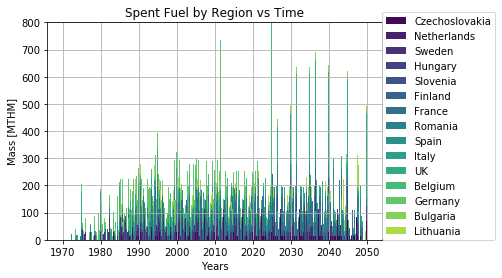
\includegraphics[width=.8\textwidth]{./images/sim_output/france/regional_snf.png}
        \end{center}
    \caption{Waste output mass is separated by their origin region.}
    \end{figure}
\end{frame}

\begin{frame}
    \frametitle{Output - Prototype analysis}
    \begin{itemize}
        \item The user can separate analysis by prototype
        \item User can see how much \texttt{power} is from SFRs compared to PWRs.
    \end{itemize}
    \begin{figure}[htbp!]
        \begin{center}
                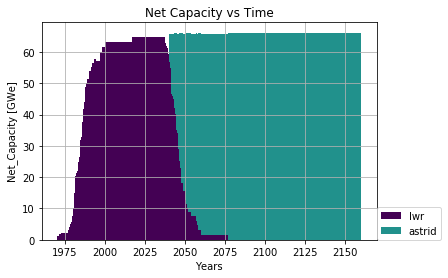
\includegraphics[width=.8\textwidth]{./images/sim_output/france/power_plot.png}
        \end{center}
    \caption{Power generation is separated by prototype (SFR, PWR).}
    \end{figure}
\end{frame}


\begin{frame}
    \frametitle{Output - Prototype analysis}
    \begin{itemize}
        \item The user can separate analysis by prototype
        \item User can see how much fuel is from which facility.
    \end{itemize}
    \begin{figure}[htbp!]
        \begin{center}
                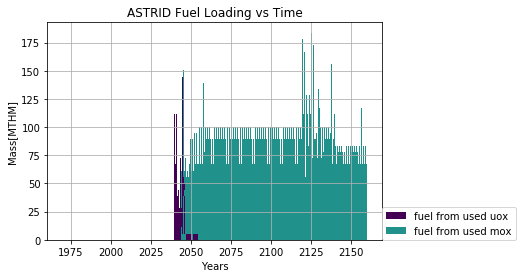
\includegraphics[width=.8\textwidth]{./images/sim_output/france/where_fuel.png}
        \end{center}
    \caption{Fuel production is separated by production facility.}
    \end{figure}
\end{frame}

\begin{frame}
    \frametitle{Sensitivity Study}
    Breeding ratio sensitivity study can be done by simply changing the 
    SFR output fuel recipe in the input file.
    \begin{figure}[htbp!]
        \begin{center}
                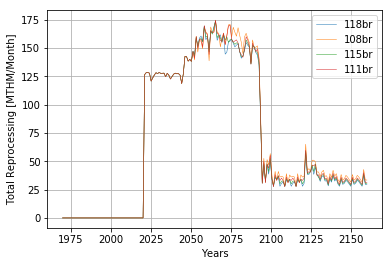
\includegraphics[width=.8\textwidth]{./images/sim_output/france/br_tot_rep.png}
        \end{center}
    \caption{Breeding Ratio affect on total reprocessing.}
    \end{figure}
\end{frame}

\begin{frame}
    \frametitle{Sensitivity Study}
    Lifetime extension sensitivity study can be done by adding the
    lifetime of the pwrs and adjusting SFR deployment accordingly.
    \begin{figure}[htbp!]
        \begin{center}
                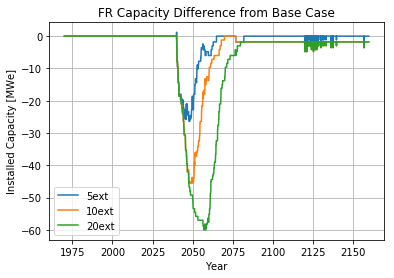
\includegraphics[width=.8\textwidth]{./images/sim_output/france/fr_diff.png}
        \end{center}
    \caption{PWR lifetime extension affect on FR installed capacity.}
    \end{figure}
\end{frame}




\subsection{Example - Predicting the past (U.S.)}

\begin{frame}
    \frametitle{Predicting the past - U.S}
    Work done by undergraduate researcher Gyutae Park and Gwendolyn Chee at the University of Illinois - Urbana Champaign.
    \begin{enumerate}
        \item Import database to construct Cyclus simulation
        \begin{enumerate}
            \item IAEA PRIS database for reactor deployment history
            \item Wikidata for Reactor coordinates
        \end{enumerate}
        \item `Predict the past' - fuel usage, power generated
        \item Demonstrate GIS capabilities of Cyclus
    \end{enumerate}
\end{frame}


\begin{frame}
    \frametitle{Example Workflow}
    Similar workflow has been used for this analysis study.
\begin{figure}
\scalebox{0.65}{
        \centering
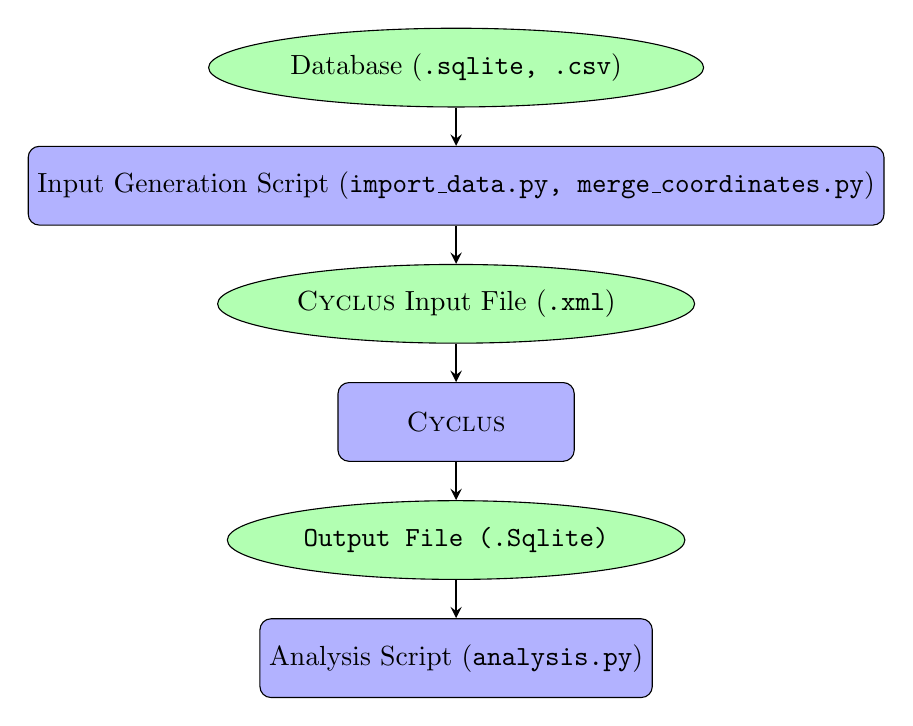
\begin{tikzpicture}[node distance=1.5cm]
\node (database) [object] {Database (\texttt{.sqlite, .csv})};
\node (script) [process, below of=database] {Input Generation Script (\texttt{import\_data.py, merge\_coordinates.py})};
\node (input) [object, below of=script] {\Cyclus Input File (\texttt{.xml})};
\node (cyclus) [process, below of=input]{\Cyclus};
\node (output) [object, below of=cyclus]{\texttt{Output File (\texttt{.Sqlite})}};
\node (script2) [process, below of=output]{Analysis Script (\texttt{analysis.py})};

\draw [arrow] (database) -- (script); 
\draw [arrow] (script) -- (input); 
\draw [arrow] (input) -- (cyclus);
\draw [arrow] (cyclus) -- (output);
\draw [arrow] (output) -- (script2);
\end{tikzpicture}
}
\caption{Green circles and blue boxes represent files and software 
processes, respectively, in the computational workflow.}
\label{diag:comp}
\end{figure}

\end{frame}

\begin{frame}
    \frametitle{Results - Fuel into reactors}
    \begin{figure}[htbp!]
        \begin{center}
                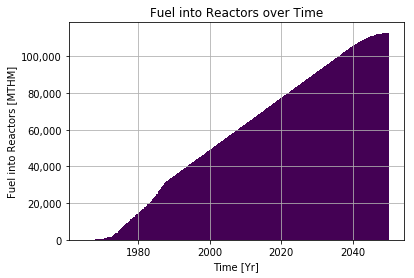
\includegraphics[width=.8\textwidth]{./images/sim_output/us/fuel.png}
        \end{center}
    \caption{Cumulative fuel into U.S. reactors over time.}
    \end{figure}
\end{frame}


\begin{frame}
    \frametitle{Results - Natural Uranium usage}
    \begin{figure}[htbp!]
        \begin{center}
                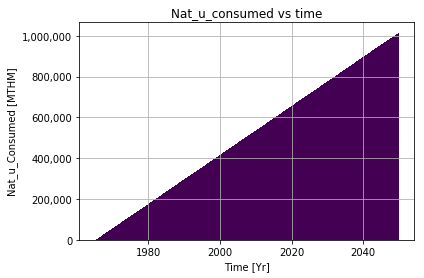
\includegraphics[width=.8\textwidth]{./images/sim_output/us/natu.png}
        \end{center}
    \caption{Cumulative natural uranium consumption in the U.S. over time.}
    \end{figure}
\end{frame}

\begin{frame}
    \frametitle{Results - Power generated}
\begin{figure}[htbp!]
\begin{minipage}[b]{.45\linewidth}
    \begin{center}
        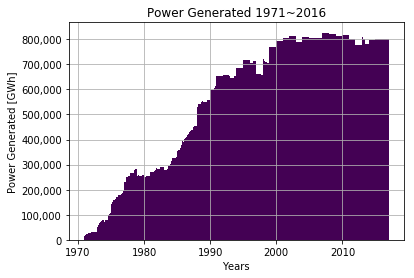
\includegraphics[width=\textwidth]{./images/sim_output/us/cyc_pow.png}
    \end{center}
    \caption{Nuclear Power generated simulated by Cyclus}
\end{minipage}
\hspace{.5cm}
\begin{minipage}[b]{.45\linewidth}
    \centering
        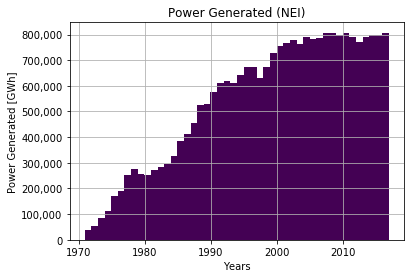
\includegraphics[width=\linewidth]{./images/sim_output/us/nei_pow.png}
    \caption{Nuclear power generation data from NEI \footnotemark}
\end{minipage}
\end{figure}
    \footnotetext{US Nuclear Generating Statistics. (n.d.). Retrieved from https://www.nei.org/Knowledge-Center/Nuclear-Statistics/US-Nuclear-Power-Plants/US-Nuclear-Generating-Statistics}
\end{frame}

\begin{frame}
    \frametitle{Results - GIS}
    \begin{figure}[htbp!]
        \begin{center}
                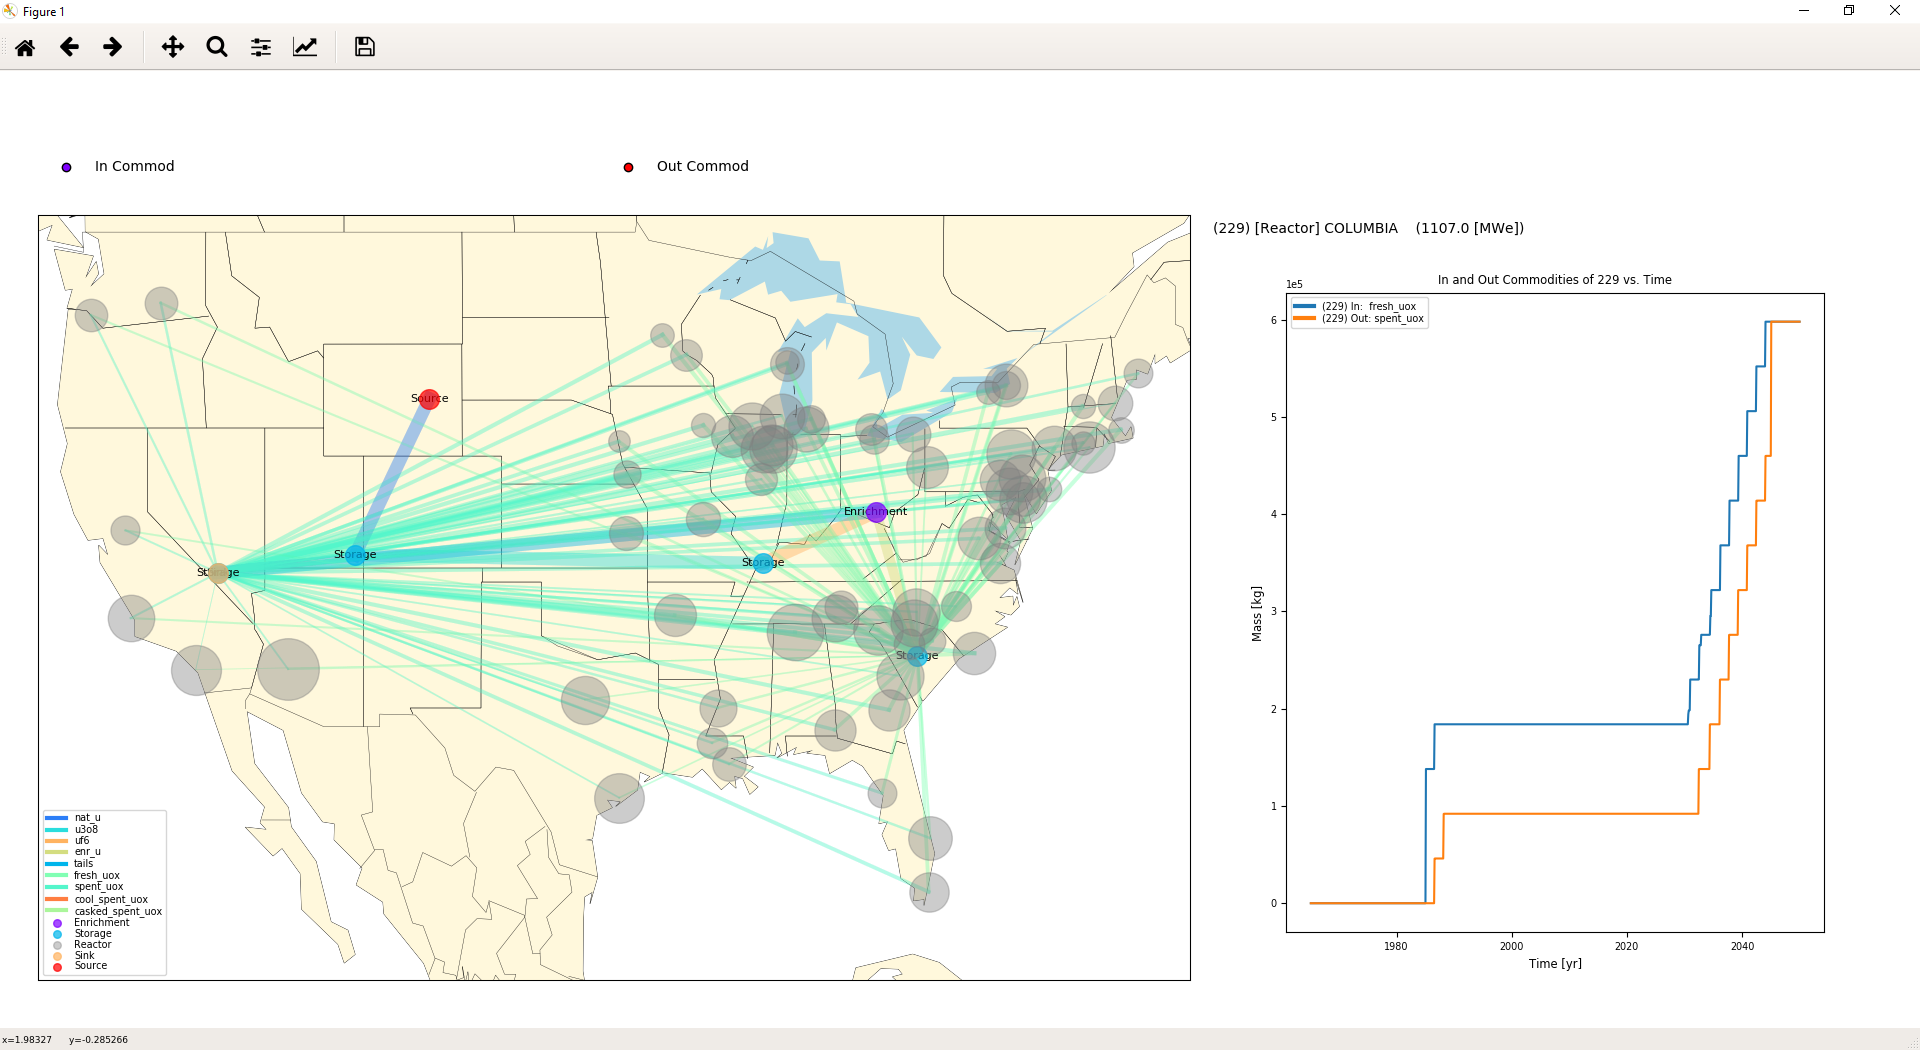
\includegraphics[width=\textwidth]{./images/sim_output/us/map.png}
        \end{center}
    \caption{Interactive map of U.S. reactors and fuel cycle
     facilities. Lines show transactions between two facilities.}
    \end{figure}
\end{frame}



\section{Conclusion}
\begin{frame}
    \frametitle{Conclusion}
    Cyclus is a performant, expanding fuel cycle simulator that holds promise for future applications. It demonstrated its capability to:
    \begin{itemize}
        \item `Predict the past'
        \item Model transition scenarios
        \item Visualize important fuel cycle metrics
    \end{itemize}
\end{frame}

\begin{frame}
    \frametitle{Future Work Ongoing}
    \texttt{Cycamore} is adequate for rough analyses, but more accurate
    modules or additional tools would increase analysis fidelity
    \begin{itemize}
        \item Dynamic archetype parameters (e.g. \texttt{refuel\_time}
                changing in time or sampled from a distribution)
        \item In-module depletion (i.e. Using in-module SERPENT Reduced-order-model)
        \item Demand-driven deployment \footnotemark
        \item Database-based MSR simulator
    \end{itemize}
    \footnotetext{NEUP 16-10512}
\end{frame}


\begin{frame}
    \frametitle{Room for Improvement}
    To really take it to the next level, a more organized, supported
    effort is needed.
    \begin{itemize}
        \item Organized / Supported Code development and Quality Assurance (QA)
        \begin{itemize}
            \item Currently done by a Cylcus Developer Manager (25\% PostDoc)
            \item User support and bug fixing on Github done voluntarily
            \item Various archetypes are outdated
        \end{itemize}
        \item Easier User Interface (UI) for broader user base
        \begin{itemize}
            \item Input generation / validation / visualization (e.g. Fulcrum)
            \item Ouput visualization / postprocessing (e.g. ORION)
        \end{itemize}
        \item Cloud execution of Cyclus (Users `submit job')
        \begin{itemize}
            \item Avoid Installation issues for end-users
        \end{itemize}
    \end{itemize}
\end{frame}


\begin{frame}
    \frametitle{Why \Cyclus?}
    \Cyclus has a unique expandable nature due to its open-source-ness and
    modularity of models. Here are a list of interesting projects we came up with:
    \begin{itemize}
        \item Central database driven high fidelity fuel cycle simulation
        \begin{itemize}
            \item Every fuel cycle facility in the Evaluation and Screening report modeled
            \item Real-life designs (Reactor designs, Reprocessing technologies etc.)
            \item plug-and-play for user
        \end{itemize}
        \item GIS-based work (every agent can have a coordinate property)
        \begin{itemize}
            \item Transportation model
            \item Energy demand / region based deployment (i.e. EAGLE-I)
        \end{itemize}
        \item Various Metrics Connector
        \begin{itemize}
        	\item Postprocessor for Safeguard / Non-proliferation metrics
        \end{itemize}
    \end{itemize}
\end{frame}


\begin{frame}
	\frametitle{Synergy with ORNL}
	\begin{itemize}
		\item Software management and QA infrastructure
		\item Computational development team with GUI development
		\item Most importantly: the personnel resources
		\begin{itemize}
			\item Fuel Cycle simulation is a combination of all aspects of nuclear engineering
			\item Insight / data from Safeguards, Reactor Physics 
			\item \textbf{Provide questions that needs to be answered}
		\end{itemize}
	\end{itemize}
\end{frame}


\begin{frame}
	\frametitle{Synergy with ORNL}
	\begin{itemize}
		\item \Cyclus is a tool. It should be developed to fulfill the needs of its customers.
		\item ORNL is an awesome resource for those interesting questions.
	\end{itemize}
\end{frame}


\begin{frame}
	\frametitle{Conclusion II}
	\begin{itemize}
		\item \Cyclus, with partnership with ORNL, can become a one-stop tool for system integration analysis.
		\item To achieve this, a central, supported effort is needed for \Cyclus
		\item Staff can `plug in' their developed model (reactor design, fuel cycle facility etc) to see the model's performance in a larger system.
	\end{itemize}
\end{frame}




\begin{frame}
    \frametitle{Acknowledgements}
    Invaluable advice and help provided by:
    Joshua Peterson-Droogh, Kathryn Huff, Andrew Worrall, Eva Davison

    This summer sponsored by:
    NESLS program at ORNL
\end{frame}

\begin{frame}
    Thank you. Questions / Concerns / Ideas?
\end{frame}
\end{document}



